First the test was made with a fixed Qinit and Qgoal. The first plot, see figure \ref{fig:l2h}, shows the distance to the human center in the path. This figure show us, the influence of the constraint behaviour. The horizontal line indicating the threshold of the constraint area. Below this horizontal line the robot tool will be inside and above it will be outside of the constraint area. We can clearly see, when the robot tool is below this horizontal line, it will move away from the human center(function is raising). Until it get above the line. Also when the robot tool is above this line, it will never get back inside of the constraint area again. 

\begin{figure}[h!]
 \centering
 \includegraphics[width=0.9\textwidth]{images/LengthToHuman.pdf}
 \caption{Plot of the distance to the human center for 10 different routes all starting in and ending in the same configurations}
 \label{fig:l2h}
\end{figure}

\section{Testing of the system with random Qinit and Qgoal configurations}
Now we had test your system with a fixed Qinit and Qgoal, to see how it would act. Now we will try with random configurations, to test the success ratio to finding a path.
Out of 2000 tests, $74.1\%$ a path was found with the algorithm. It means, we got 1481 found paths. A Histogram plot of theirs length can be seen on figure \ref{fig:hyp}. 

\begin{figure}[h!]
 \centering
 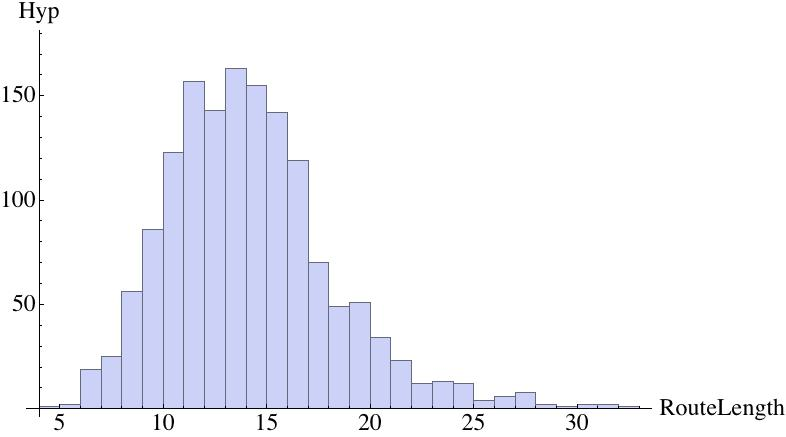
\includegraphics[width=0.8\textwidth]{images/Hyp.jpg}
 \caption{Histogram of the length of a route from a random point ending in a random point in in the configuration space}
 \label{fig:hyp}
\end{figure}

At last a histogram of the number of iterations is shown, see figure \ref{fig:k}. The algorithm was taking in average before a path was found. An iteration includes an EXTEND on one of the trees and CONNECT of the another tree. 
Figure \ref{fig:k} shows the result and it shows that most of the time the path was found in first iteration. It means only one random jump was made before a directly path was able to be made. So the choice of K = 50, for this scene.

\begin{figure}[h!]
 \centering
 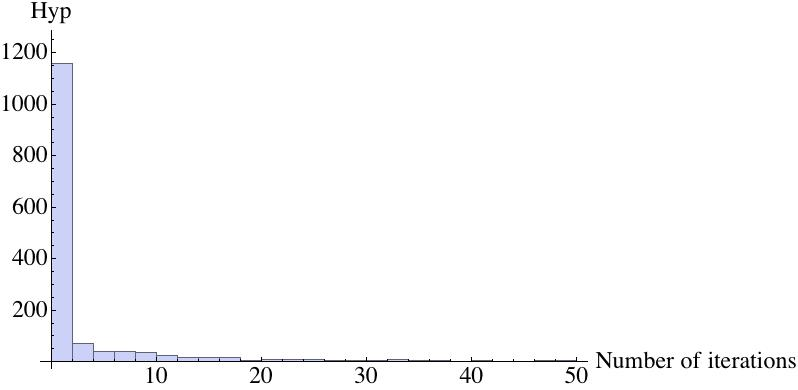
\includegraphics[width=0.8\textwidth]{images/K.jpg}
 \caption{Histogram of the number of iterations in the main loop of algorithm before a solution was found}
 \label{fig:k}
\end{figure}